\subsection{Lệnh pingpong}
\underline{\textbf{Chức năng của lệnh:}} Lệnh \verb|pingpong| thực hiện việc truyền 1 byte dữ liệu giữa hai tiến trình bằng một cặp \textbf{pipe} (\textbf{pipe} là một đường dẫn dữ liệu giữa hai tiến trình, với một đầu được cố định để đọc dữ liệu từ thiết bị nhập và đầu còn lại ghi dữ liệu ra \linebreak thiết bị xuất) \cite{mit-xv6}.

\underline{\textbf{Thiết lập thuật toán:}}
\begin{enumerate}[labelindent=1em, labelsep=0.2cm, leftmargin=1cm, wide=\parindent, topsep=0.1cm, itemsep=-1ex, partopsep=1.5ex, parsep=1.5ex]
	\item Khởi tạo hai \textbf{pipe} \verb|p_in| và \verb|p_out| và phân chia tiến trình ra làm hai bằng hàm \verb|fork()|. Tiến trình con (\verb|fork() == 0|) dùng \verb|p_in| để đọc dữ liệu và truyền qua tiến trình cha. Tiến trình cha (\verb|fork() > 0|) dùng \verb|p_out| làm điều tương tự với tiến trình con.
	\item Tiến trình con truyền 1 byte dữ liệu (trong mã nguồn dùng chữ \verb|'i'|) cho tiến trình cha. Tiến trình cha sau khi nhận được thì in số thứ tự của nó và thông báo \verb|received ping|.
	\item Tiến trình cha truyền 1 byte dữ liệu (trong mã nguồn dùng chữ \verb|'o'|) cho tiến trình con. Tiến trình con sau khi nhận được thì in số thứ tự của nó và thông báo \verb|received pong|.
\end{enumerate}

Lệnh sẽ báo lỗi khi người dùng nhập sai cú pháp.

Dưới đây là kết quả chạy thử trên \verb|qemu| và kiểm tra lệnh \verb|pingpong| bằng chương trình kiểm thử:
\begin{figure}[htp!]
	\centering
	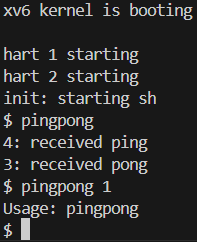
\includegraphics[width=0.5\textwidth]{figures/exec-pingpong}
	\caption{Kết quả chạy thử \textbf{pingpong} trên \textbf{qemu}}
\end{figure}
\begin{figure}[htp!]
	\centering
	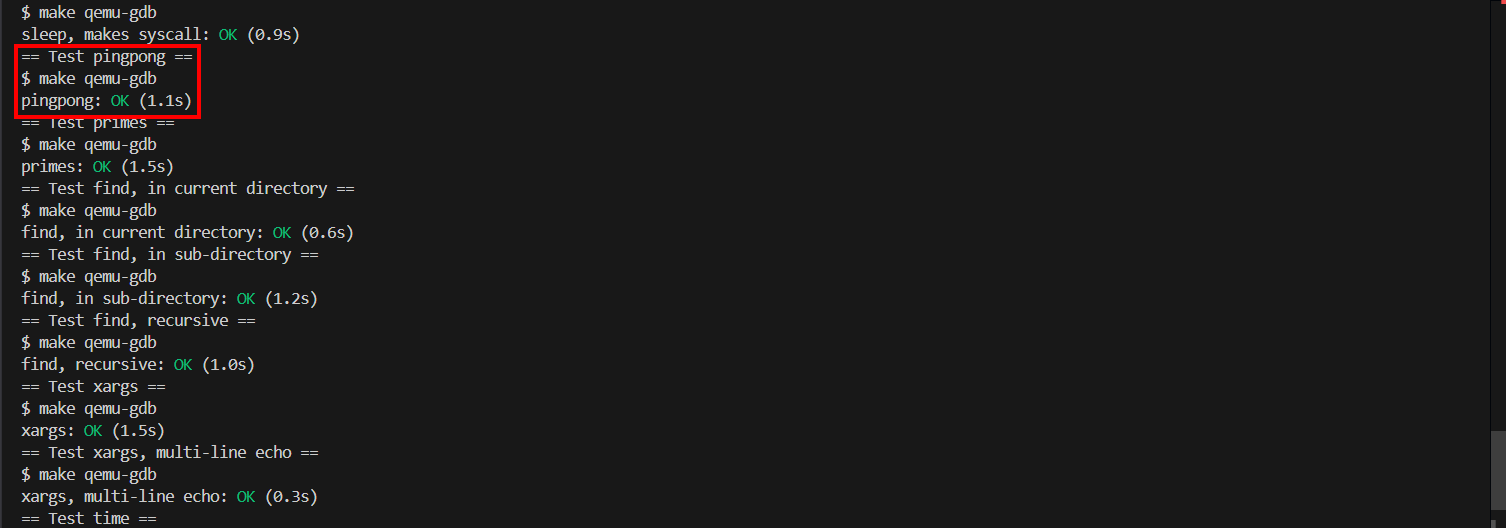
\includegraphics[width=0.9\textwidth]{figures/pingpong-test}
	\caption{Kết quả kiểm thử \textbf{pingpong} bằng công cụ chấm bài \textbf{grade} của MIT}
\end{figure}